\section{Introduction}

When researchers hope to begin drafting a thesis, chapter, report, or paper, they frequently lean toward using \LaTeX, which is a typesetting system that is commonly used to prepare technical and scientific documents \cite{latex}.
\LaTeX\ separates the authors' content from the rules that define the document's formatting.
This allows publishers and editors to maintain or enforce consistency in formatting without affecting the textual content of the documents.

While \LaTeX\ eases the editorial process for publishers, it requires authors to learn its syntax and semantics.
This burden is especially visible for first-time or occasional users, who s manage markup while also developing the content of their work.

In parallel, large language models (LLMs) and generative artificial intelligence (GenAI) have become powerful productivity tools across many domains.
However, in academic contexts, the adoption of GenAI provokes ethical issues.
Many scholars worry that using GenAI tools may compromise academic integrity, be it through inadvertent plagiarism or hallucinated citations and claims.

This report introduces Spartan Write, an AI-powered document authoring platform designed for scholars and researchers preparing academic reports, articles, papers, and theses.
Spartan Write addresses this tension by locating a middle ground, where AI can assist academic writing \textit{without} the ethical pitfalls of general-purpose GenAI.
The key principle guiding Spartan Write is this: \textbf{the tool only works with content that the author provides}. It does not generate, hallucinate, or synthesise new claims, arguments, or evidence.
Instead, it focuses entirely on the technical and structural aspects of academic writing—formatting, organisation, and presentation.

At its core, Spartan Write pairs an intelligent agent with \LaTeX, offloading the effort of editing and refining documents through natural conversation.
The agent assists with structuring tables, managing figure placement and captions, handling LaTeX formatting, and organising user-provided content, all without requiring users to write raw markup.
The agent is built to never generate content.
Instead, users provide all the content, and the agent handles the mechanical work of translating that into proper academic formatting and structure.
Spartan Write provides hand-curated document templates spanning common types of documents, like thesis reports and journal papers.
The result is a program that lets researchers focus on their content while AI handles the technical details.
Figure \ref{fig:authoring-workflow} depicts the improvement proposed by Spartan Write to the authoring workflow.

\begin{figure}[htbp]
    \centering
    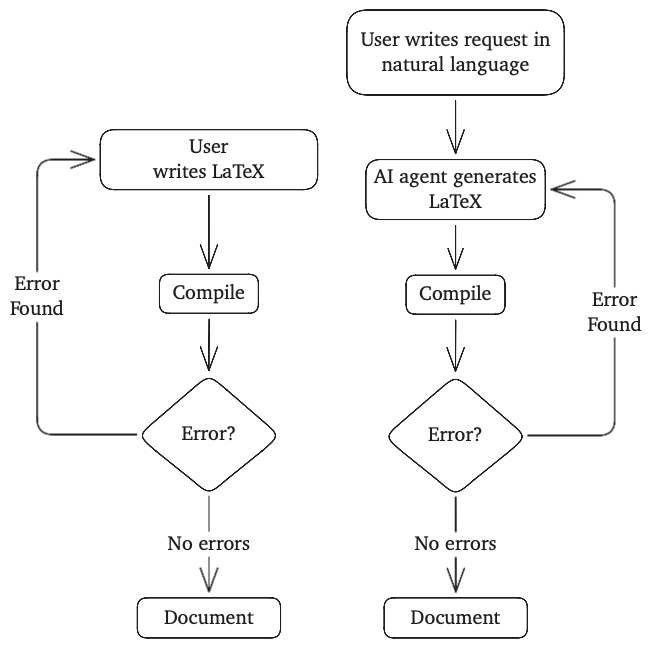
\includegraphics[width=.9\linewidth]{figures/authoring-workflow.excalidraw.png}
    \caption{Manual and agent-assisted \LaTeX\ authoring loops}
    \label{fig:authoring-workflow}
\end{figure}
